\section{Problem Setting}\label{sec:setting}

A \emph{scene} $Z$ consists of a view graph $\mathcal{G}=(\mathcal{V},\mathcal{E})$ with $n=|\mathcal{V}|$ cameras and $m=|\mathcal{E}|$ edges, an observed relative rotation $\tilde R_{ij}\in SO(3)$ for every edge $(i,j)$, and a native uncertainty $\hat\sigma_{ij}>0$ supplied by the front end (a two-view solver, a learned matcher, or a feed-forward network such as VGGT~\cite{wang2025vggt} or MASt3R~\cite{leroy2024mast3r}). The unknown absolute rotations $R_i$ map world to camera coordinates, and the noise-free model is $R_{ij}=R_jR_i^{\top}$. We write $\angle(R)=\arccos\big((\operatorname{tr}R-1)/2\big)$ for the geodesic angle and $\operatorname{Log}:SO(3)\to\mathbb{R}^3$ for the rotation vector. An edge is an \emph{inlier} when $\angle(\tilde R_{ij}R_{ij}^{\top})\le\tau$ for a fixed $\tau$ (we use $\tau=5^\circ$ on real data; in simulation the generator labels outliers). Rotation averaging returns estimates $\hat R_i$, defined up to a global gauge $R_i\mapsto R_iG$, and the per-camera error $e_i=\angle(\hat R_i G^\star R_i^{\top})$ is measured after the best robust gauge alignment $G^\star$.

We ask for three outputs in addition to $\{\hat R_i\}$: (i) edge gates whose expected loss of inlier edges is controlled at user levels; (ii) a registration set $\mathcal{V}_{\mathrm{reg}}\subseteq\mathcal{V}$ that excludes cameras whose pose is not supported by consistent evidence; and (iii) a bound $B_i$ for every registered camera such that the expected fraction of registered cameras with $e_i>B_i$ is at most $\alpha_{\mathrm{cam}}$. We also want (i) and (iii) to remain close to their targets when the test scene is noisier than the calibration scenes, without labels from the test scene.

\paragraph*{Statistical model} Calibration uses scenes with reference rotations. We assume that calibration scenes and the test scene are exchangeable (for example, drawn i.i.d.\ from a distribution over scenes). This is a statement about \emph{scenes}; edges and cameras inside a scene may be arbitrarily dependent. For shifted test scenes we use the following first-order model.

\begin{assumption}[Scale shift]\label{ass:scale}
A shifted scene is generated as $\tilde R_{ij}=R_jR_i^{\top}\operatorname{Exp}(\rho^\star\eta_{ij})$ on inlier edges, where $\{\eta_{ij}\}$ follows the calibration noise law and $\rho^\star\ge 1$ is an unknown scalar; outlier edges are arbitrary. Native uncertainties $\hat\sigma_{ij}$ are \emph{not} rescaled, i.e.\ the front end is unaware of the shift.
\end{assumption}

Assumption~\ref{ass:scale} models what the 2026 calibration audit of feed-forward reconstruction models reports: confidences keep their ranking but their level is wrong, and the error of the level changes with the data~\cite{deng2026audit}. Fog, rain, low light or a new sensor increase error at a fixed reported confidence.

\section{Method}\label{sec:method}

\begin{figure*}[!htbp]
\centering
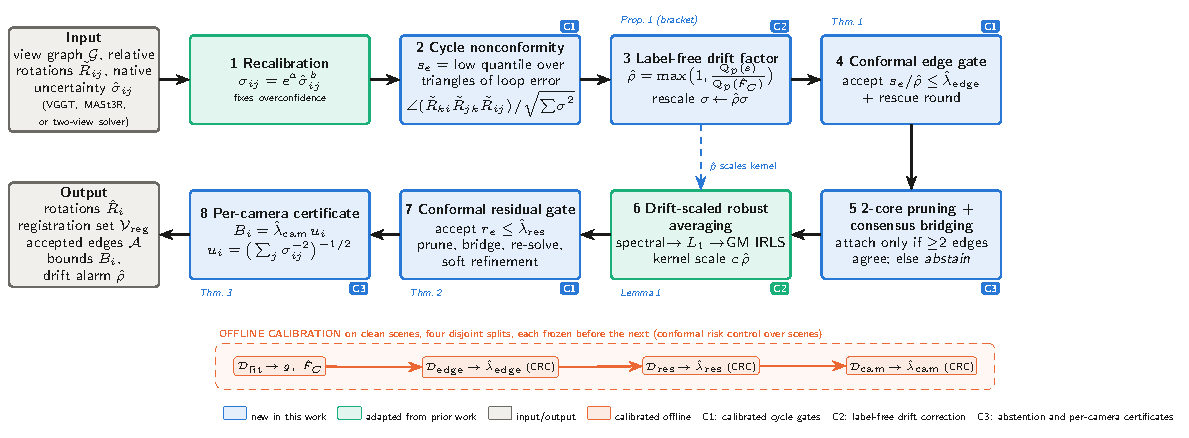
\includegraphics[width=\textwidth]{figs/pipeline.pdf}
\caption{The CARA pipeline. Blue blocks are new in this work and green blocks adapt prior components; tags C1--C3 map blocks to the three contributions and italic labels to the guarantees of \cref{sec:theory}. Offline, four disjoint calibration splits fix the recalibration map $g$ and reference law $\hat F_C$ (used by blocks 1 and 3) and the thresholds $\hat\lambda_{\mathrm{edge}}$, $\hat\lambda_{\mathrm{res}}$ and $\hat\lambda_{\mathrm{cam}}$ (used by blocks 4, 7 and 8). Online, the drift factor $\hat\rho$ from block 3 rescales the uncertainties and the robust kernel of block 6.}
\label{fig:pipeline}
\end{figure*}

\Cref{fig:pipeline} shows the pipeline and \cref{alg:cara} summarizes it. Each step below states its purpose and the design choice that matters for the guarantees.

\subsection{Recalibrated edge uncertainty}
Native uncertainties from learned front ends are rank-informative but overconfident~\cite{deng2026audit}. We fit a two-parameter power law $\sigma_{ij}=g(\hat\sigma_{ij})=e^{a}\hat\sigma_{ij}^{\,b}$ by least squares on $\log\angle(\tilde R_{ij}R_{ij}^\top)$ versus $\log\hat\sigma_{ij}$ over inlier edges of a fitting split $\mathcal{D}_{\mathrm{fit}}$. The constant $e^{a}$ does not affect the calibrated gates and bounds, which are scale-free; it only sets the units of the fixed bridging threshold $\beta$ below. When the front end supplies no uncertainty (as on the 1DSfM data), $\sigma_{ij}$ is constant.

\subsection{Cycle nonconformity score}
For an edge $e=(i,j)$ and a third camera $k$ with edges $(j,k)$ and $(k,i)$, the cycle $C_{ijk}=\tilde R_{ki}\tilde R_{jk}\tilde R_{ij}$ equals the identity for consistent data. We normalize its angle by the predicted cycle spread and aggregate over at most $K$ triangles with a \emph{low} quantile:
\begin{equation}\label{eq:score}
s_e=\operatorname{Q}_{q}\Big\{\frac{\angle(C_{ijk})}{\sqrt{\sigma_{ij}^2+\sigma_{jk}^2+\sigma_{ki}^2}}\;:\;k\in\mathcal{T}_e\Big\},\qquad q=0.25.
\end{equation}
The low quantile protects an inlier edge from triangles contaminated by outliers on the other two edges: with an outlier rate $\varepsilon$, a triangle is clean with probability $(1-\varepsilon)^2$, which is $0.42$ at $\varepsilon=0.35$, so a median would often land on a contaminated triangle. The price is that a group of \emph{mutually consistent} wrong edges passes the test; \cref{sec:dop} measures this failure mode. Edges without any triangle get $s_e=\mathrm{NaN}$ and are deferred to the residual gate.

\subsection{Label-free drift factor}
Let $F_C$ be the law of inlier scores on calibration scenes ($\rho=1$) and $\hat F_C$ its empirical version on $\mathcal{D}_{\mathrm{fit}}$. On a test scene with scores $\{s_e\}$ we estimate
\begin{align}
\hat\rho_{\mathrm{pt}}&=\max\Big(1,\frac{\operatorname{Q}_{p}(\{s_e\})}{\operatorname{Q}_{p}(\hat F_C)}\Big),\quad p=0.2,\label{eq:rho}\\
\hat\rho_{\mathrm{safe}}&=\max\Big(1,\frac{\operatorname{Q}_{p'}(\{s_e\})}{\operatorname{Q}_{(p'-\bar\varepsilon)/(1-\bar\varepsilon)}(\hat F_C)}\Big),\label{eq:rhosafe}
\end{align}
with $p'=0.5$ and $\bar\varepsilon=0.4$, and rescale $\sigma_{ij}\leftarrow\hat\rho\,\sigma_{ij}$, $s_e\leftarrow s_e/\hat\rho$. Cycle closure needs no reference poses, so $\hat\rho$ is computed from the test scene alone. The point estimate uses a low quantile, which is dominated by inliers; the safe estimate is an upper bound on $\rho^\star$ at the population level whenever the outlier fraction is at most $\bar\varepsilon$ (\cref{prop:bracket}). $\hat\rho$ is also a scene-level alarm: $\hat\rho\gg1$ means that the front end's confidence is not valid for this scene.

\subsection{Conformal edge gate}
An edge is accepted in round one if $s_e\le\hat\lambda_{\mathrm{edge}}$ or $s_e=\mathrm{NaN}$. In round two we recompute \eqref{eq:score} using only triangles whose other two edges were accepted, and \emph{rescue} edges whose clean-triangle score falls below $\hat\lambda_{\mathrm{edge}}$. Round two only adds edges, so it cannot increase the loss controlled in \cref{thm:edge}. The threshold $\hat\lambda_{\mathrm{edge}}$ is set by conformal risk control~\cite{angelopoulos2024crc} on a split $\mathcal{D}_{\mathrm{edge}}$ with the per-scene loss
\begin{equation}\label{eq:edgeloss}
L^{\mathrm{edge}}_Z(\lambda)=\frac{1}{|\mathcal{I}_Z|}\sum_{e\in\mathcal{I}_Z}\mathbb{1}[s_e>\lambda],
\end{equation}
where $\mathcal{I}_Z$ is the set of cycle-testable inlier edges of $Z$:
\begin{equation}\label{eq:crc}
\hat\lambda=\inf\Big\{\lambda:\ \tfrac{N}{N+1}\hat R_N(\lambda)+\tfrac{1}{N+1}\le\alpha\Big\},
\end{equation}
with $\hat R_N(\lambda)=\frac1N\sum_{t=1}^{N}L_{Z_t}(\lambda)$ the average loss over the $N$ calibration scenes.

\subsection{Core pruning and consensus bridging}
Gating can leave cameras attached by one or two edges that cannot be checked against anything else. We therefore take the $2$-core of the accepted graph: cameras with fewer than two accepted edges are detached, repeatedly. A detached component $C$ returns to the main component $M$ only through \emph{consensus}: we solve $C$ and $M$ separately, each rejected edge $(a,b)$ with $a\in M$, $b\in C$ implies a gauge $G_{ab}=\hat R_b^{C\top}\tilde R_{ab}\hat R_a^{M}$, and $C$ is attached if at least two such gauges agree, $\angle(G_{ab}^{\top}G_{a'b'})/\sqrt{\sigma_{ab}^2+\sigma_{a'b'}^2}\le\beta$ with a fixed $\beta=3$. Otherwise the cameras of $C$ \emph{abstain} and are reported as unregistered, which is the behavior of incremental SfM when registration fails~\cite{schoenberger2016sfm}. A simpler alternative, ``connect-back'', re-adds the best-scoring rejected edges until the graph is connected; it attaches components through unverified edges and causes catastrophic errors (\supp{2}).

\subsection{Drift-scaled robust averaging}
On the main component we run spectral chordal initialization~\cite{martinec2007robust}, $L_1$-IRLS and Geman--McClure IRLS (GM-IRLS)~\cite{chatterjee2018robust} in the Lie algebra~\cite{govindu2004lie}, with prior weights $w_{ij}\propto\sigma_{ij}^{-2}$ clipped to their 5th--95th percentiles and a kernel scale $c\,\hat\rho$ with $c=5^\circ$. Scaling the kernel with $\hat\rho$ makes the IRLS weights, which depend on $r_{ij}/(c\hat\rho)$, invariant to the noise level under \cref{ass:scale} (\cref{lem:equiv}); the clipped prior weights prevent a single confidently wrong edge from dominating, which is what happens when native confidences enter averaging unmodified (\cref{sec:synth}).

\subsection{Conformal residual gate and final refinement}
After the first solve we compute whitened residuals $r_{ij}=\angle(\hat R_j^{\top}\tilde R_{ij}\hat R_i)/\sigma_{ij}$ for all edges, accept $r_{ij}\le\hat\lambda_{\mathrm{res}}$ (calibrated by \eqref{eq:crc} on a split $\mathcal{D}_{\mathrm{res}}$ with the analogous loss), repeat pruning and bridging, and re-solve. A final Geman--McClure pass over \emph{all} edges among registered cameras, started from the gated solution, recovers inlier redundancy that the hard gates removed. This pass, the pruning and the bridging are outside the guarantees of \cref{sec:theory}.

\subsection{Per-camera certificates}
For a registered camera, $u_i=\big(\sum_{j:(i,j)\in\mathcal{E}_{\mathrm{acc}}}\sigma_{ij}^{-2}\big)^{-1/2}$ is the standard deviation of a Gaussian information proxy. Its scale is wrong for the same reasons as $\hat\sigma$, so we calibrate it: on a split $\mathcal{D}_{\mathrm{cam}}$ we set $\hat\lambda_{\mathrm{cam}}$ by \eqref{eq:crc} with the loss
\begin{equation}\label{eq:camloss}
L^{\mathrm{cam}}_Z(\lambda)=\frac{1}{|\mathcal{V}_{\mathrm{reg}}|}\sum_{i\in\mathcal{V}_{\mathrm{reg}}}\mathbb{1}[e_i>\lambda u_i],
\end{equation}
and report $B_i=\hat\lambda_{\mathrm{cam}}u_i$. Because $u_i$ is built from the $\hat\rho$-scaled $\sigma_{ij}$, the bound widens by $\hat\rho$ on a shifted scene.

\subsection{Extensions for camera-level failures}\label{sec:ext}
A learned front end can misread a whole image: every relative rotation that involves camera $i$ then carries the same error $D_i$, $\tilde R_{ij}=R_{ij}D_i^{\top}$ (or $D_iR_{ij}$ when $i$ is the second index). Such errors cancel in every cycle, $\tilde R_{ki}\tilde R_{jk}\tilde R_{ij}=D_i\,(R_{ki}R_{jk}R_{ij})\,D_i^{\top}$ is conjugate to the true cycle and has the same angle, so no cycle test can detect them and camera $i$ is registered with a wrong pose. A scalar drift factor does not describe them either. We add two optional components that act only on the per-camera bounds; the rotations, gates and registration set are unchanged.

\paragraph*{E1: failure-aware calibration} The calibration scenes are augmented with modeled failures before $\hat\lambda_{\mathrm{cam}}$ is set. Each scene of $\mathcal{D}_{\mathrm{cam}}$ and $\mathcal{D}_{\mathrm{fit}}$ enters five times: unchanged; with inlier edges amounting to 10\% and 20\% of all its edges replaced by uniformly random rotations whose confidences are drawn from the confidences of real outlier edges in $\mathcal{D}_{\mathrm{fit}}$; and with 10\% and 20\% of its cameras misread by a common rotation of $20^\circ$ to $180^\circ$ (plus per-edge noise with $3^\circ$ per axis). The threshold is then the CRC threshold over the augmented $\mathcal{D}_{\mathrm{cam}}$; with E2, $\hat\beta$ and the group boundaries are fitted on the augmented $\mathcal{D}_{\mathrm{fit}}$.

\paragraph*{E2: difficulty-conditional bounds} The normalizer $u_i$ uses only the confidences of the accepted edges. We replace it by
\begin{equation}\label{eq:vnorm}
v_i=u_i\exp\big(\hat\beta^{\top}[1,\,x_i]\big),
\end{equation}
where $x_i$ collects four label-free features of camera $i$ in the final solution: the log median whitened residual of its accepted edges, the fraction of its edges that were rejected, the median log confidence of its edges relative to the scene median, and the log number of accepted edges (the residual is floored at $0.05$ and the exponent in \eqref{eq:vnorm} is clipped to $[-5,5]$). $\hat\beta$ is the least-squares fit of $\log(e_i/u_i)$ on $\mathcal{D}_{\mathrm{fit}}$. The registered cameras are split into $G=3$ groups by $\log v_i$, with group boundaries fixed on $\mathcal{D}_{\mathrm{fit}}$, and each group $g$ receives its own threshold $\hat\lambda_{\mathrm{cam}}^{(g)}$, calibrated by \eqref{eq:crc} over the scenes of $\mathcal{D}_{\mathrm{cam}}$ that have registered cameras in that group, with the loss restricted to those cameras. The bound is $B_i=\hat\lambda^{(g(i))}_{\mathrm{cam}}v_i$. A bound above $30^\circ$ is reported as a \emph{flag}: the method then declares the camera unreliable instead of certifying it. \Cref{sec:v2} evaluates E1 and E2 together with three further extensions: an edge uncertainty learned from several front-end signals (E3), a larger evaluation over all 13 ETH3D scenes (E4), and the effect on camera positions after translation averaging (E5).

\subsection{Calibration protocol}
The four splits $\mathcal{D}_{\mathrm{fit}},\mathcal{D}_{\mathrm{edge}},\mathcal{D}_{\mathrm{res}},\mathcal{D}_{\mathrm{cam}}$ are disjoint. $\mathcal{D}_{\mathrm{fit}}$ fixes $g$ and $\hat F_C$; each later split is processed by the pipeline with all earlier quantities frozen. This ordering is what makes the loss on the test scene exchangeable with the losses on the split that calibrates it. We use $|\mathcal{D}_{\mathrm{fit}}|=20$ and $40$ scenes for each other split; with $N=40$, the term $1/(N+1)$ in \eqref{eq:crc} is $0.024$. Calibration scenes are clean ($\rho^\star=1$).

\begin{algorithm}[t]
\caption{CARA on one test scene}\label{alg:cara}
\begin{algorithmic}[1]
\Require $\mathcal{G}$, $\{\tilde R_{ij},\hat\sigma_{ij}\}$; calibration $(g,\hat F_C,\hat\lambda_{\mathrm{edge}},\hat\lambda_{\mathrm{res}},\hat\lambda_{\mathrm{cam}})$
\State $\sigma_{ij}\gets g(\hat\sigma_{ij})$; compute $s_e$ by \eqref{eq:score}
\State $\hat\rho\gets$ \eqref{eq:rho} or \eqref{eq:rhosafe}; $\sigma\gets\hat\rho\sigma$; $s\gets s/\hat\rho$
\State $\mathcal{A}\gets\{e: s_e\le\hat\lambda_{\mathrm{edge}}\ \text{or}\ s_e=\mathrm{NaN}\}$; rescue with clean-triangle scores
\State $\mathcal{A}\gets$ 2-core$(\mathcal{A})$; consensus bridging $\Rightarrow\mathcal{A},\mathcal{V}_{\mathrm{reg}}$
\State $\hat R\gets$ spectral $\to L_1$-IRLS $\to$ GM-IRLS on $\mathcal{A}$, weights clip$(\sigma^{-2})$, kernel $c\hat\rho$
\State $\mathcal{A}\gets\{e:r_e\le\hat\lambda_{\mathrm{res}}\}$; 2-core; bridging; re-solve
\State GM-IRLS on all edges within $\mathcal{V}_{\mathrm{reg}}$, initialized at $\hat R$
\State $u_i\gets(\sum_{\mathcal{A}\ni(i,j)}\sigma_{ij}^{-2})^{-1/2}$; $B_i\gets\hat\lambda_{\mathrm{cam}}u_i$
\State \Return $\hat R$, $\mathcal{V}_{\mathrm{reg}}$, $\mathcal{A}$, $\{B_i\}$, $\hat\rho$
\end{algorithmic}
\end{algorithm}

\paragraph*{Complexity} Measured runtimes are in \supp{4}. Triangle enumeration costs $O(\sum_{(i,j)}\min(d_i,d_j))$ with $d_i$ the degree, and scoring costs $O(mK)$. Each IRLS iteration solves a sparse $n\times n$ Laplacian system three times (one per axis). Spectral initialization is a dense eigendecomposition for $3n\le1500$ and a Lanczos solve otherwise. Bridging solves each detached component once per attachment.
